\section{From $G_{\mathcal{P}, n}(\alpha, \nu)$ to $G_{\mathcal{P}}(\alpha, \nu)$ (Proving Proposition \ref{prop:convergence_average_clustering_P_n})}\label{sec:clustering_Pn_to_P}

Now that we have a complete picture of the behavior of the local clustering coefficient and function in the limit model $G_\Pcal$ we will proceed to relate this to the clustering in the hyperbolic model $G_{\H,n}$. The first step is to relate the clustering in the infinite model to that of the finite box model $G_{\Pcal, n}$. Recall that $G_{\Pcal,n}$ is obtained by restricting the Poisson Point Process $\PPP$ to the box $\Rcal_n = (-I_n, I_n] \times (0, R_n]$, with $I_n = \frac{\pi}{2} e^{R_n/2}$ (we write $\Pcal_n$ for this process), and connecting two points $p_1, p_2 \in \Rcal_n$ if $|x_1 - x_2|_{\pi e^{R_n/2}} \le e^{(y_1 + y_2)/2}$ where we identified the left and right boundary of $\Rcal_n$. See Section~\ref{ssec:finite_model} for more details. 

In this section we shall compute the asymptotic difference between triangle counts in the finite and infinite model. First we recall the definition of $\Kcal_{C}(k_n)$
\[
	\Kcal_C(k_n) = \left\{p \in \R : \frac{k_n - C \kappa_n}{\xi_{\alpha,\nu}} \vee 0 \le e^{\frac{y}{2}}
	\le \frac{k_n + C \kappa_n}{\xi_{\alpha,\nu}} \wedge e^{R_n/2} \right\},	
\]
with
\[
	\kappa_n := \begin{cases}
		\log(n) &\mbox{if } k_n = \bigT{1},\\
		\sqrt{k_n \log(k_n)} &\mbox{else.}
	\end{cases}
\]
In addition we note that the function $\phi_n(y)$ in Lemma~\ref{lem:average_degree_P_n} satisfies
\[
	\phi_n(y) = \bigT{e^{-(\alpha - \frac{1}{2})(R_n - y)}},
\]
which yields the following useful corollary to Lemma~\ref{lem:average_degree_P_n}.

\begin{corollary}\label{cor:average_degree_P_n_K}
Let $\alpha > \frac{1}{2}$, $C > 0$ and $k_n$ be any sequence satisfying $k_n = \smallO{n^{\frac{1}{2\alpha - 1}}}$. Then, for all $p \in \Kcal_{C}(k_n)$,
\[
	\mu_{\alpha,\nu ,n}(B_{\Pcal,n}(p)) = \mu_{\alpha,\nu}(B_\Pcal(p))\left(1 - \bigT{k_n^{2\alpha - 1} n^{-(2\alpha - 1)}}\right).
\]
\end{corollary}


\subsection{Comparing triangles between $G_\Pcal(\alpha,\nu)$ and $G_{\Pcal,n}(\alpha,\nu)$}

We now turn to the task of calculating the expected number of triangles of a node at height $y$, for both the infinite model and the finite box model. Let $p_0 = (0,y)$ and recall that 
\[
	\Exp{T_{\Pcal,n}(p_0)} = \frac{1}{2}\iint_{\Rcal_n^2} T_{\Pcal,n}(p_0,p_1,p_2)
	f_{\alpha,\nu}(x_1,y_1) f_{\alpha,\nu}(x_1,y_1) \, dx_1 \, dx_2 \, dy_1 \, dy_2,
\]
where
\[
	T_{\Pcal,n}(p_0,p_1,p_2) = \ind{p_1 \in B_{\Pcal,n}(p)}\ind{p_2 \in B_{\Pcal,n}(p)}\ind{p_2 \in B_{\Pcal,n}(p_1)}.
\]

The difference between the indicator $\ind{p_1 \in B_{\Pcal,n}(p)}$ in the finite box model and $\ind{p_1 \in B_{\Pcal}(p)}$ is that in $G_{\Pcal,n}(\alpha,\nu)$ we identified the boundaries of the interval $[-\frac{\pi}{2}e^{R_n/2}, \frac{\pi}{2} e^{R_n/2}]$. It is clear that for any $0 \le y \le R_n$ we have that $\BallPon{p_0} = \BallPo{p_0} \cap \Rcal_n$. However, when we take another point $p^\prime \in \BallPon{p}$ then it could happen that there are points in the intersection $\BallPon{p} \cap \BallPon{p^\prime}$ that are not in $\BallPo{p} \cap \BallPo{p^\prime}$. Let us denote this region by $\mathcal{T}_{\Pcal \Delta \Pcal_n}(p,p^\prime)$. Then, any $p_2 \in \mathcal{T}_{\Pcal \Delta \Pcal_n}(p,p^\prime)$ creates a triangle with $p$ and $p^\prime$ in $G_{\Pcal,n}(\alpha,\nu)$ that is not present in $G_{\Pcal}(\alpha, \nu)$.  

Define
\begin{equation}\label{eq:def_tilde_triangle_indicator}
	\widetilde{T}_{\Pcal,n}(p_0,p_1,p_2) = \ind{p_1 \in B_{\Pcal,n}(p)}\ind{p_2 \in B_{\Pcal,n}(p)}\ind{p_2 \in B_{\Pcal}(p_1) \cap \Rcal_n}
\end{equation}
Then
\[
	\sum_{p_1,p_2 \in \Pcal_n \setminus (0,y)}^{\ne} T_{\Pcal,n}(p_0,p_1,p_2) - \widetilde{T}_{\Pcal,n}(p_0,p_1,p_2)
	= \sum_{p_1,p_2 \in \Pcal_n \setminus (0,y)}^{\ne} \ind{p_1 \in \BallPon{p_0}} \ind{p_2 \in \mathcal{T}_{\Pcal \Delta \Pcal_n}(p_0,p_1)},
\]
where the sums are over all distinct pairs $(p_1, p_2) \in \Pcal_n \setminus \{(0,y)\}$.

\begin{figure}[!t]
\centering
\begin{tikzpicture}
	%Define the coordinates 
	%p = (\u,\v) and p^\prime = (\uu, \vv)
	%Box \Rcal_n has width 2\r and height \t
	\pgfmathsetmacro{\u}{0} %0
	\pgfmathsetmacro{\v}{1} %1
	\pgfmathsetmacro{\uu}{1.4} %1.4
	\pgfmathsetmacro{\vv}{0.8} %0.8
	\pgfmathsetmacro{\r}{6}
	\pgfmathsetmacro{\t}{4}
	
	%The box \Rcal_n
	\draw[line width=1pt] (-\r,0) -- (\r,0) -- (\r,\t) -- (-\r,\t) -- (-\r,0);

	%Dram both nodes
    \draw node[fill, circle, inner sep=0pt, minimum size=5pt] (p1) at (\u,\v) {};
    \path (p1)+(-0.2,0.2) node {$p$};
    \draw node[fill,blue, circle, inner sep=0pt, minimum size=5pt] (p2) at (\uu,\vv) {};
    \path (p2)+(-0.2,0.2) node {\color{blue}$p^\prime$};
	
	
	%Boundaries p = (\u,\v)
	
	%Right boundary
	\pgfmathsetmacro{\rightbounduv}{\u+exp((\v)/2)}
	\draw[domain=\rightbounduv:\r,smooth,variable=\x,black,line width=1pt] plot (\x, {2*ln(\x)-\v});
    %Left boundary
    \pgfmathsetmacro{\leftbounduv}{\u-exp((\v)/2)}
    \draw[domain=\leftbounduv:-\r,smooth,variable=\x,black,line width=1pt] plot (\x, {2*ln(-\x)-\v});
    
    %Boundaries p^\prime = (\uu,\vv)
    
    %Right boundary
    \pgfmathsetmacro{\rightbounduuvv}{\uu+exp((\vv)/2)}
    \draw[domain=\rightbounduuvv:\r,smooth,variable=\x,blue,line width=1pt] plot (\x, {2*ln(\x-\uu)-\vv});
    %Shifted right boundary
    \pgfmathsetmacro{\shiftrightbounduuvv}{\uu+exp((\vv + \t)/2)-2*\r}
    \draw[domain=\shiftrightbounduuvv:-\r,smooth,variable=\x,blue,line width=1pt] plot (\x, {2*ln(\x+(2*\r-\uu))-\vv});
    %Left boundary 
    \pgfmathsetmacro{\leftbounduuvv}{\uu-exp((\vv)/2)}
    \draw[domain=\leftbounduuvv:-\r,smooth,variable=\x,blue,line width=1pt] plot (\x, {2*ln(\uu-\x)-\vv});
    %Shifted left boundary
    \pgfmathsetmacro{\shiftleftbounduuvv}{\uu-exp((\vv + \t)/2)+2*\r}
    \draw[domain=\shiftleftbounduuvv:\r,smooth,variable=\x,blue,line width=1pt] plot (\x, {2*ln(2*\r + \uu-\x)-\vv});
    
    %Define x^\ast(p^\prime) and y^\ast(p^\prime)
    \pgfmathsetmacro{\uuast}{\uu-\r}
    \pgfmathsetmacro{\vvast}{2*ln(\r)-\vv}
    
    %Define intersection left black and shifted blue curve
    \pgfmathsetmacro{\vast}{2*ln((2*\r - \uu)/(exp(\v/2) + exp(\vv/2)))}
    \pgfmathsetmacro{\uast}{(\uu - 2*\r)/(1 + exp((\vv - \v)/2))}    
   
    %Define h_1(p) = h_2(p)
    \pgfmathsetmacro{\hp}{2*ln(\r-\u)-\v}
    
    %Define h_1(p^\prime) and h_2(p^\prime)
    \pgfmathsetmacro{\hh}{2*ln(\uu+\r)-\vv}
    \pgfmathsetmacro{\hhh}{2*ln(\r-\uu)-\vv}
    
    %Highlight area between left black, left blue and shifted right blue line
	\draw[red,line width=1pt,pattern=north west lines, pattern color=red] 
		plot[domain=\uuast:\uast,smooth,variable=\x,red] (\x, {2*ln(\x+(2*\r-\uu))-\vv}) 
		-- 
		plot[domain=\uast:-\r,smooth,variable=\x,red] (\x, {2*ln(-\x)-\v})
		-- 
		(-\r,\hh)
		-- 
		plot[domain=-\r:\uuast,smooth,variable=\x,red] (\x, {2*ln(\uu-\x)-\vv});
	
%	\draw node[fill, circle, inner sep=0pt, minimum size=4pt, blue] at (\uuast,\vvast) {};
%	\draw node[fill, circle, inner sep=0pt, minimum size=4pt, black] at (\uast,\vast) {};
%	\draw node (f1) at (\uuast,\vvast+0.9) {\color{blue}$(x^\ast(p^\prime), y^\ast(p^\prime))$};
%	\draw node (f2) at (\uast+1,\vast-1.25) {\color{black}$(\hat{x}(p,p^\prime), \hat{y}(p,p^\prime))$};
%	
%	\draw[->,thick] (f2) -- (\uast+0.1,\vast-0.2);
%	\draw[->,thick,blue] (f1) -- (\uuast,\vvast+0.2);
	
	 \draw[dashed,line width=1pt,blue] (\uuast,0) -- (\uuast,\vvast);
	 \draw node at (\uuast+0.1,-0.4) {\color{blue}$x^\ast(p^\prime)$};
	 \draw[dashed,line width=1pt,blue] (\r,\vvast) -- (\uuast,\vvast);
	 \draw node at (\r+0.75,\vvast) {\color{blue}$y^\ast(p^\prime)$};
	 \draw[dashed,black,line width=1pt] (-\r,\vast) -- (\uast,\vast);
	 \draw node at (-\r-0.75,\vast) {\color{black}$\hat{y}(p,p^\prime)$};
	 \draw[dashed,black,line width=1pt] (\uast,\vast) -- (\uast,0);
	 \draw node at (\uast-0.1,-0.4) {\color{black}$\hat{x}(p,p^\prime)$};
	 
	 \draw node[fill, circle, inner sep=0pt, minimum size=4pt, blue] at (\uuast,\vvast) {};
	 \draw node[fill, circle, inner sep=0pt, minimum size=4pt, black] at (\uast,\vast) {};
	
    \draw node at (-\r-0.75,\hh+0.1) {\color{blue}$h_1(p^\prime)$};
    \draw node at (\r+0.75,\hhh-0.1) {\color{blue}$h_2(p^\prime)$};

\end{tikzpicture}
\caption{Example configuration of two points $p$ and $p^\prime$ for which $\BallPon{p} \cap \BallPon{p^\prime}$ is not a subset of $\BallPo{p} \cap \BallPo{p^\prime}$. The red region indicates the area of points belonging to $\BallPon{p} \cap \BallPon{p^\prime}$ but not to $\BallPo{p} \cap \BallPo{p^\prime}$.}
\label{fig:comparing_triangles_diff_intersections}
\end{figure}

Figure \ref{fig:comparing_triangles_diff_intersections} shows an example of a configuration where $\mathcal{T}_{\Pcal \Delta \Pcal_n}(p,p^\prime) \ne \emptyset$. We observe that $\mathcal{T}_{\Pcal \Delta \Pcal_n}(p,p^\prime) \ne \emptyset$ because the right boundary of the ball $\BallPon{p^\prime}$ exists the right boundary of the box $\Rcal_n$ and then, since we identified the boundaries, continues from the left so that $\BallPon{p^\prime}$ covers part of the ball $\BallPon{p}$ which would not be covered in the infinite limit model. 

To further analyze this, let us introduce some notation. For any $p = (x,y) \in \Rcal_n$ we will define the left and right boundary functions as, respectfully,
\begin{align}
	b_p^-(z) &= \begin{cases}
		2 \log\left(x-z\right) - y &\mbox{if }  -\frac{\pi}{2} e^{R_n/2} \le z \le x - e^{y/2}  \\
		2\log\left(\pi e^{R_n/2} + x - z\right) - y 
			&\mbox{if } x - e^{(y + R_n)/2} + \pi e^{R_n/2} \le z \le \frac{\pi}{2} e^{R_n/2}\\
		0 &\mbox{else}
	\end{cases}\\
	b_p^+(z) &= \begin{cases}
		2 \log\left(z-x\right) - y &\mbox{if } x + e^{y/2} \le z \le \frac{\pi}{2} e^{R_n/2} \\
		2\log\left(\pi e^{R_n/2} + z - x\right) - y 
			&\mbox{if } -\frac{\pi}{2} e^{R_n/2} \le z \le x + e^{(y + R_n)/2} - \pi e^{R_n/2}\\
		0 &\mbox{else}
	\end{cases}
\end{align}
Note that these functions describe the boundaries of the ball $\BallPon{p}$. In particular, $p^\prime \in \BallPon{p}$ if and only if $y^\prime \ge \min\left\{b_p^-(x^\prime), b_p^+(x^\prime)\right\}$.

For the remainder of the analysis we restrict ourselves to the case where $x^\prime > 0$. Due to symmetry the situation for $x^\prime < 0$ is the same. There are two important points in the box $\Rcal_n$. These are the intersection between the left boundary of $p^\prime$ and the right boundary of $p^\prime$, as it continues from the left side of the box, and the left boundary of $p$. We denote by $(x^\ast(p^\prime), y^\ast(p^\prime))$ the intersection between the left and right boundary of $p^\prime$ and by $(\hat{x}(p,p^\prime), \hat{y}(p,p^\prime))$ the intersection between the left boundary of $p$ and the right boundary of $p^\prime$, see Figure \ref{fig:comparing_triangles_diff_analysis}. After some simple algebra we obtain the following expressions for the coordinates of these two points
\begin{align*}
	x^\ast(p^\prime) &= x^\prime - \frac{\pi}{2} e^{R_n/2}\\
	y^\ast(p^\prime) &= 2\log\left(\frac{\pi}{2}e^{R_n/2}\right) - y^\prime\\
	\hat{x}(p,p^\prime) &= \frac{x^\prime - \pi e^{R_n/2}}{1 + e^{(y^\prime - y)/2}} \\
	\hat{y}(p,p^\prime) &= 2 \log\left(\frac{\pi e^{R_n/2} - x^\prime}{e^{y/2} + e^{y^\prime/2}}\right)
\end{align*}

The crucial observation is that $\mathcal{T}_{\Pcal \Delta \Pcal_n} = \emptyset$ as long as the point $(x^\ast(p^\prime), y^\ast(p^\prime))$ is above the left boundary of $p$. This happens exactly when $y^\ast(p^\prime) > b_p^-(x^\ast(p^\prime))$. Therefore the boundary of this event is given by the equation $y^\ast(p^\prime) = b_p^-(x^\ast(p^\prime))$ which reads
\[
	2\log\left(\frac{\pi}{2}e^{R_n/2}\right) - y^\prime = 2\log\left(\frac{\pi}{2} e^{R_n/2} -x^\prime\right) - y.
\]
Solving this equation gives us the function
\begin{equation}
	b^\ast_p(z) = y - 2\log\left(1 - \frac{z}{\frac{\pi}{2} e^{R_n/2}}\right),
\end{equation}
which is displayed by the red curve in Figure \ref{fig:comparing_triangles_diff_analysis}. It holds that $y^\ast(p^\prime) > b_p^-(x^\ast(p^\prime))$ if and only if $y^\prime < b^\ast_p(x^\prime)$ and hence we have that $\mathcal{T}_{\Pcal \Delta \Pcal_n} = \emptyset$ for all $p^\prime \in \Rcal_n$ for which $y^\prime \ge b^\ast_p(x^\prime)$. We also not that when $y^\prime = b^\ast_p(x^\prime)$ the two points $(x^\ast(p^\prime), y^\ast(p^\prime))$ and $(\hat{x}(p,p^\prime),\hat{y}(p,p^\prime))$ coincide.



\begin{figure}[!t]

\centering
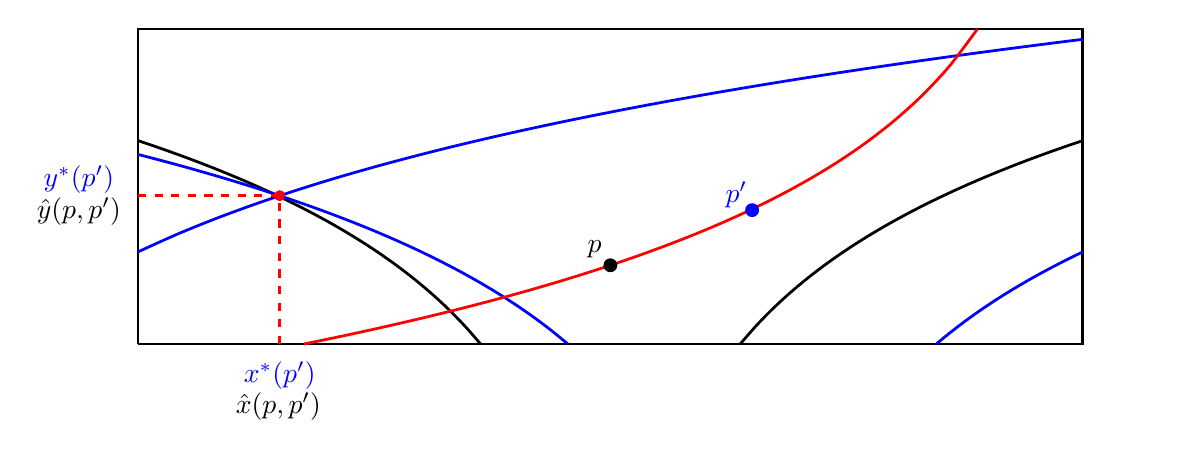
\begin{tikzpicture}
	%Define the coordinates 
	%p = (\u,\v) and p^\prime = (\uu, \vv)
	%Box \Rcal_n has width 2\r and height \t
	\pgfmathsetmacro{\u}{0}
	\pgfmathsetmacro{\v}{1}
	\pgfmathsetmacro{\uu}{1.8}
	\pgfmathsetmacro{\vv}{1.7}
	\pgfmathsetmacro{\r}{6}
	\pgfmathsetmacro{\t}{4}
	
	%The box \Rcal_n
	\draw[line width=1pt] (-\r,0) -- (\r,0) -- (\r,\t) -- (-\r,\t) -- (-\r,0);	
	
	%Boundaries p = (\u,\v)
	
	%Right boundary
	\pgfmathsetmacro{\rightbounduv}{\u+exp((\v)/2)}
	\draw[domain=\rightbounduv:\r,smooth,variable=\x,black,line width=1pt] plot (\x, {2*ln(\x)-\v});
    %Left boundary
    \pgfmathsetmacro{\leftbounduv}{\u-exp((\v)/2)}
    \draw[domain=\leftbounduv:-\r,smooth,variable=\x,black,line width=1pt] plot (\x, {2*ln(-\x)-\v});
    
    %Boundaries p^\prime = (\uu,\vv)
    
    %Right boundary
    \pgfmathsetmacro{\rightbounduuvv}{\uu+exp((\vv)/2)}
    \draw[domain=\rightbounduuvv:\r,smooth,variable=\x,blue,line width=1pt] plot (\x, {2*ln(\x-\uu)-\vv});
    %Shifted right boundary
    \pgfmathsetmacro{\shiftrightbounduuvv}{\uu+exp((\vv + \t)/2)-2*\r}
    %\draw[domain=\shiftrightbounduuvv:-\r,smooth,variable=\x,blue,line width=1pt] plot (\x, {2*ln(\x+(2*\r-\uu))-\vv});
    \draw[domain=-\r:\r,smooth,variable=\x,blue,line width=1pt] plot (\x, {2*ln(\x+(2*\r-\uu))-\vv});
    %Left boundary 
    \pgfmathsetmacro{\leftbounduuvv}{\uu-exp((\vv)/2)}
    \draw[domain=\leftbounduuvv:-\r,smooth,variable=\x,blue,line width=1pt] plot (\x, {2*ln(\uu-\x)-\vv});
    %Shifted left boundary

    
    %Star boundary
    \pgfmathsetmacro{\starleftbound}{\r*(1-exp(\v/2))}
    \pgfmathsetmacro{\starrightbound}{\r*(1-exp((\v-\t)/2))}
    \draw[domain=\starleftbound:\starrightbound,smooth,variable=\x,red, line width=1pt] plot (\x, {2*ln((\r/(\r-\x)))+\v});
    
    %Define h_1(p) = h_2(p)
    \pgfmathsetmacro{\hp}{2*ln(\r-\u)-\v}
%    \draw node at (\r+0.75,\hp) {\color{black}$h(y)$};
    \draw node at (\r+1,\hp) {};
    
    %Define h_1(p^\prime) and h_2(p^\prime)
    \pgfmathsetmacro{\hh}{2*ln(\uu+\r)-\vv}
    \pgfmathsetmacro{\hhh}{2*ln(\r-\uu)-\vv}

%    \draw node at (-\r-0.75,\hh+0.1) {\color{blue}$h_1(p^\prime)$};
%    \draw node at (\r+0.75,\hhh) {\color{blue}$h_2(p^\prime)$};
    
    %Define x^\ast(p^\prime) and y^\ast(p^\prime), intersection of left and shifted right blue curve
    \pgfmathsetmacro{\uuast}{\uu-\r}
    \pgfmathsetmacro{\vvast}{2*ln(\r)-\vv}

    %Define intersection left black and shifted blue curve
    \pgfmathsetmacro{\vast}{2*ln((2*\r - \uu)/(exp(\v/2) + exp(\vv/2)))}
    \pgfmathsetmacro{\uast}{(\uu - 2*\r)/(1 + exp((\vv - \v)/2))} 

%    \draw[dashed,thick,black] (-\r,\hhh) -- (\r,\hhh);
    \draw[dashed,line width=1pt,red] (\uuast,0) -- (\uuast,\vvast);
    \draw node at (\uuast,-0.4) {\color{blue}$x^\ast(p^\prime)$};
    \draw[dashed,line width=1pt,red] (-\r,\vvast) -- (\uuast,\vvast);
    \draw node at (-\r-0.75,\vvast+0.2) {\color{blue}$y^\ast(p^\prime)$};
%    \draw[dashed,black,line width=1pt] (-\r,\vast) -- (\uast,\vast);
    \draw node at (-\r-0.75,\vast-0.2) {\color{black}$\hat{y}(p,p^\prime)$};
%    \draw[dashed,black,line width=1pt] (\uast,\vast) -- (\uast,0);
    \draw node at (\uast,-0.8) {\color{black}$\hat{x}(p,p^\prime)$};
    
    \draw node[fill, circle, inner sep=0pt, minimum size=4pt, red] at (\uuast,\vvast) {};
    
   	%Draw both nodes
    \draw node[fill, circle, inner sep=0pt, minimum size=5pt] (p1) at (\u,\v) {};
    \path (p1)+(-0.2,0.2) node {$p$};
    \draw node[fill,blue, circle, inner sep=0pt, minimum size=5pt] (p2) at (\uu,\vv) {};
    \path (p2)+(-0.2,0.2) node {\color{blue}$p^\prime$};
    
    
    
%    \draw node[fill, circle, inner sep=0pt, minimum size=4pt, black] at (\uast,\vast) {};
    
%    \draw node at (-7,2.5835) {$h(y)$};

    
%    \draw[dotted,thick,black] (4.5208,2.0174) -- (4.5208,0);
%    \draw[dotted,thick,black] (4.5208,2.0174) -- (6,2.0174);
    
%    \draw node at (4.5208,-0.5) {$w_x(p,p^\prime)$};
%    \draw node at (7,2.0174) {$w_y(p,p^\prime)$};
    
%    \draw node at (0,3.5) {\color{blue}$x_1 = x^\prime + e^{\frac{y^\prime + y_1}{2}}$};
%    \draw node at (-2,1.6) {\color{blue}$x_1 = x^\prime - e^{\frac{y^\prime + y_1}{2}}$};
%    \draw node at (-4.5,1) {$x_1 = x - e^{\frac{y + y_1}{2}}$};
%    \draw node at (2,1.5) {$x_1 = x + e^{\frac{y + y_1}{2}}$};

\end{tikzpicture}
\caption{???.}
\label{fig:comparing_triangles_diff_analysis}
\end{figure}

This analysis allows us to compute the expected difference in the number of triangles for $\Pcal$ and $\Pcal_n$, for a node with height $y$. 

\begin{lemma}\label{lem:clustering_error_T_term}
Let $(k_n)_{n \ge 1}$ be any sequence such that $k_n = \smallO{n^{\frac{1}{2\alpha + 1}}}$. Then, for some $C > 0$ and $p \in \Kcal_{C}(k_n)$, as $n \to \infty$,
\[
	\int_{\Rcal_n} \mu_{\alpha, \nu}\left(\mathcal{T}_{\Pcal \Delta \Pcal_n}(p,p_1)\right) f_{\alpha, \nu}(x_1,y_1) 
	\dd x_1 \dd y_1 = \bigO{y n^{-(2\alpha - 1)} + n^{-(2\alpha-1)} e^{y}}
\]
\end{lemma}

The proof of the lemma is not difficult but cumbersome, since it involves computing many different integrals. We postpone this proof till the end of this section and proceed with the main goal, proving Proposition~\ref{prop:convergence_average_clustering_P_n}. But first we state a small lemma about the scaling of $s_\alpha(k_n)$ that will be very useful.  

\begin{lemma}\label{lem:scaling_s_alpha}
Let $s_\alpha(k_n)$ be as defined in \eqref{eq:def_scaling_function}. Then for any $k_n = \smallO{n^{\frac{1}{2\alpha + 1}}}$, as $n \to \infty$,
\[
	n^{-(2\alpha - 1)} = \smallO{s_\alpha(k_n)}.
\]
\end{lemma}

\begin{proof}
First let $\frac{1}{2} < \alpha < \frac{3}{4}$. Then
\[
	n^{-(2\alpha - 1)}s_\alpha(k_n)^{-1} = n^{-(2\alpha -1)}k_n^{4\alpha - 2}
	= \smallO{n^{-(2\alpha - 1) + \frac{4\alpha - 2}{2\alpha + 1}}} 
	= \smallO{n^{-\frac{4\alpha^2 - 4\alpha + 1}{2\alpha + 1}}}
	= \smallO{1},
\]
since $4\alpha^2 - 4\alpha + 1 > 0$ for all $\alpha > \frac{1}{2}$. Similarly, for $\alpha \ge \frac{3}{4}$ we have
that $4\alpha^2 > 2$ and hence,
\[
	n^{-(2\alpha - 1)} s_{\alpha}(k_n) = \smallO{n^{-(2\alpha - 1)} k_n} = \smallO{n^{-\frac{4\alpha^2 - 2}{2\alpha + 1}}}
	= \smallO{1}.
\]
\end{proof}

\begin{proof}[Proof of Proposition~\ref{prop:convergence_average_clustering_P_n}]

Recall that
\[
	\Exp{c_{\Pcal,n}^\ast(k_n)} = \frac{\int_{\Rcal_n} \Exp{\ind{D_{\Pcal,n}(y) = k_n} T_{\Pcal,n}(y)} f_{\alpha,\nu}(x,y) \dd x \dd y}{\binom{k_n}{2}\Exp{N_{\Pcal,n}(k_n)}}.
\]
By Lemma~\ref{lem:average_degree_P_n} and a concentration argument
\[
	\Exp{N_{\Pcal,n}(k_n)} = (1+o(1)) \alpha n \int_{0}^\infty \rho(y,k_n) e^{-\alpha} \dd y 
	= (1+\smallO{1}) n \Exp{N_{\Pcal}(k_n)},
\]
and since $\Exp{\ind{D_{\H,n}(y) = k_n} T_{\Pcal,n}(y)} \le \rho_n(y,k_n) k_n^2$ another concentration argument yields
\begin{align*}
	&\hspace{-30pt}\int_{\Rcal_n} \Exp{\ind{D_{\H,n}(y) = k_n} T_{\Pcal,n}(y)} 
		f_{\alpha,\nu}(x,y) \dd x \dd y\\
	&= (1+\smallO{1})\int_{\Kcal_C(k_n)} \rho_n(y,k_n) \Exp{T_{\Pcal,n}(y)} f_{\alpha,\nu}(x,y) \dd x \dd y\\
	&= (1 + \smallO{1}) \alpha n \int_{a_n^-}^{a_n^+} \rho_n(y,k_n) \Exp{T_{\Pcal,n}(y)} e^{-\alpha} \dd x \dd y,
\end{align*}
with $a_n^\pm = 2\log\left(\frac{k_n \pm C \kappa_n}{\xi_{\alpha,\nu}}\right)$. Next we note that for $a_n^- \le y \le a_n^-$,
\[
	\Exp{T_\Pcal(y)} = \frac{\Mu{\BallPo{y}}^2}{2} \Delta_\Pcal(y) = (1+\smallO{1}) \binom{k_n}{2} \Delta_\Pcal(y)
\]
and hence it now suffices to show that
\[
	\binom{k_n}{2}^{-1}\int_{a_n^-}^{a_n^+} \rho_n(y,k_n) \Exp{T_{\Pcal,n}(y)} e^{-\alpha y} \dd y
	= (1+\smallO{1}) \int_{a_n^-}^{a_n^+} \rho(y,k_n) \Delta_\Pcal(y) e^{-\alpha y} \dd y. 
\]


We do this in two stages. First we prove that
\begin{equation}\label{eq:transition_clustering_main_term}
	\int_{a_n^-}^{a_n^+} \rho_{n}(y,k_n) \Delta_{\Pcal}(y) e^{-\alpha y} \dd y
	= (1 + \smallO{1}) \int_{a_n^-}^{a_n^+} \rho(y,k_n) \Delta_{\Pcal}(y) e^{-\alpha y} \dd y.
\end{equation}
Then we show that
\begin{equation}\label{eq:transition_clustering_error_term}
	\binom{k_n}{2}^{-1} \int_{a_n^-}^{a_n^+} \rho_n(y,k_n) \left|\Exp{T_{\Pcal,n}(y) - T_{\Pcal}(y)}\right| 
	e^{-\alpha y} \dd y
	= \smallO{1} \int_{a_n^-}^{a_n^+} \rho(y,k_n) \Delta_{\Pcal}(y) e^{-\alpha y} \dd y.
\end{equation}

Since $h(y) := \Delta_\Pcal(y)$ is uniformly bounded \eqref{eq:transition_clustering_main_term} follows directly from the second statement in Lemma~\ref{lem:concentration_argument_rho_approximation}.

For the error term~\eqref{eq:transition_clustering_error_term} we write
\begin{align*}
	\left|T_{\Pcal,n}(p) - T_{\Pcal}(p)\right| = \sum_{p_1, p_2 \in \Rcal_n} \ind{p_1 \in \BallPon{p}} \ind{p_2 \in \mathcal{T}_{\Pcal \Delta \Pcal_n}(p, p_1)} + \sum_{p_1, p_2 \in \Rcal \setminus \Rcal_n} T_{\Pcal}(p,p_1,p_2)
\end{align*}
so that by the Campbell-Mecke formula~\eqref{eq:def_Campbell-Mecke}
\begin{align*}
	\left|\Exp{T_{\Pcal,n}(p) - T_{\Pcal}(p)}\right|
	&\le \int_{\Rcal_n} \mu_{\alpha, \nu}\left(\mathcal{T}_{\Pcal \Delta \Pcal_n}(p,p_1)\right) f_{\alpha, \nu}(x_1,y_1) 
		\dd x_1 \dd y_1\\
	&\hspace{10pt}+ \iint_{\Rcal \setminus \Rcal_n} T_{\Pcal}(p,p_1,p_2) f_{\alpha, \nu}(x_1,y_1) f_{\alpha, \nu}(x_2,y_2)
		\dd x_2 \dd y_2 \dd x_1 \dd y_1. 
\end{align*}

The first integral was taken care of in Lemma \ref{lem:clustering_error_T_term}. For the second integral we have
\begin{align*}
	&\hspace{-30pt}\iint_{\Rcal \setminus \Rcal_n} T_{\Pcal}(p,p_1,p_2) f_{\alpha, \nu}(x_1,y_1) f_{\mu, \nu}(x_2,y_2)
		\dd x_2 \dd y_2 \dd x_1 \dd y_1\\
	&\le \left(\int_{\Rcal \setminus \Rcal_n} \ind{p_1 \in \BallPo{p}} f_{\alpha, \nu}(x_1,y_1) \dd x_1 \dd y_1\right)^2\\
	&= \bigO{\left(e^{y/2} \int_{R_n}^\infty e^{-(\alpha - \frac{1}{2})y_1} \dd y_1\right)^2}
		= \bigO{e^y n^{-(2\alpha - 1)}},
\end{align*}
from which we conclude that
\[
	\left|\Exp{T_{\Pcal,n}(p) - T_{\Pcal}(p)}\right| = \bigO{y n^{-(2\alpha - 1)} + n^{-(2\alpha-1)} e^{y}}
	= \bigO{n^{-(2\alpha-1)} e^{y}}.
\]
Therefore 
\begin{align*}
	&\hspace{-30pt}\binom{k_n}{2}^{-1}\int_{a_n^-}^{a_n^+} \rho(y,k_n) \left|\Exp{T_{\Pcal,n}(p) - T_{\Pcal}(p)}\right| 
		e^{-\alpha} \dd y\\
	&= \bigO{1} n^{-(2\alpha - 1)} \int_{0}^\infty \rho(y,k_n) f_{\alpha,\nu}(x,y) \dd y\\
	&= \bigO{1} n^{-(2\alpha - 1)} k_n^{-(2\alpha + 1)} = \smallO{s_\alpha(k_n) k_n^{-(2\alpha + 1)} },
\end{align*}
where the last part follows from Lemma~\ref{lem:scaling_s_alpha}. To finish the argument we observe that
\begin{align*}
	\int_{a_n^-}^{a_n^+} \rho(y,k_n) \Delta_\Pcal(y) e^{-\alpha} \dd y
	&= \bigT{1} \Exp{N_{\Pcal}(k_n)} c_\infty(k_n) = \bigT{ s_\alpha(k_n) k_n^{-(2\alpha + 1)}}.
\end{align*}
\end{proof}

Observe that the proof of Proposition~\ref{prop:convergence_average_clustering_P_n} yields the following two corollaries, which will be useful later on in Section~\ref{sec:concentration_c_P_n}.

\begin{corollary}\label{cor:adjusted_triangle_counting_P_n}
Let $\alpha > \frac{1}{2}$, $\nu > 0$ and $k_n$ be a positive sequence such that $k_n = \smallO{n^{\frac{1}{2\alpha + 1}}}$. Then, uniformly for all $p \in \Kcal_C(k_n)$, as $n \to \infty$
\[
	\Exp{\widetilde{T}_{\Pcal,n}(p)} = (1+\smallO{1})\Exp{T_\Pcal(p)},
\]
where
\[
	\widetilde{T}_{\Pcal,n}(p) = \sum_{(p_1, p_2) \in \Pcal\setminus p}^{\ne} 
		\ind{p_1 \in B_{\Pcal,n}(p)}\ind{p_2 \in B_{\Pcal,n}(p)}\ind{p_2 \in B_{\Pcal}(p_1) \cap \Rcal_n}.
\]

In particular,
\[
	\binom{k_n}{2}^{-1}\int_{\Kcal_{C}(k_n)} \rho_n(y,k_n) \Exp{\widetilde{T}_{\Pcal,n}(y)} f_{\alpha,\nu}(x,y) \dd x \dd y
	= (1+\smallO{1}) \int_{\Rcal_n} \rho(y,k_n) \Delta_\Pcal(y) f_{\alpha, \nu}(x,y) \dd x \dd y. 
\]
\end{corollary}

\subsection{Counting missing triangles}

We now come back to computing the expected number of triangles attached to node at height $y$ in $G_{\Pcal,n}(\alpha,\nu)$ that are not present in $G_{\Pcal}(\alpha,\nu)$. 

\begin{figure}[!t]

\centering
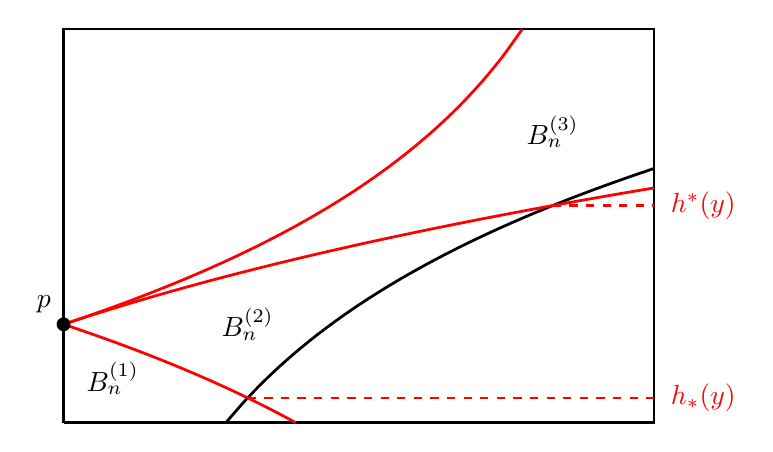
\begin{tikzpicture}[scale=1.25]

%%%%%%%%%%%%%%%%%%%%%%%%%%%%%%%%%%%%%%%%%%%%%%%%%%%%%%%%%%%%%%%%%%%%%%%%%%%%%%%%%%%%%%%%%%%%%%%%%%%
%																								  %
%	Shows the three different areas B_n^{(i)} for the computations in Lemma 					  %
%	\label{lem:clustering_error_T_term}			  												  %
%																								  %
%%%%%%%%%%%%%%%%%%%%%%%%%%%%%%%%%%%%%%%%%%%%%%%%%%%%%%%%%%%%%%%%%%%%%%%%%%%%%%%%%%%%%%%%%%%%%%%%%%%

	%Define the coordinates 
	%p = (\u,\v) and p^\prime = (\uu, \vv)
	%Box \Rcal_n has width 2\r and height \t
	\pgfmathsetmacro{\u}{0}
	\pgfmathsetmacro{\v}{1}
	\pgfmathsetmacro{\uu}{1.8}
	\pgfmathsetmacro{\vv}{1.7}
	\pgfmathsetmacro{\r}{6}
	\pgfmathsetmacro{\t}{4}
	
	%The box \Rcal_n only positive x
	\draw[line width=1pt] (0,0) -- (\r,0) -- (\r,\t) -- (0,\t) -- (0,0);	
	
	%Boundaries p = (\u,\v)
	
	%Right boundary
	\pgfmathsetmacro{\rightbounduv}{\u+exp((\v)/2)}
	\draw[domain=\rightbounduv:\r,smooth,variable=\x,black,line width=1pt] plot (\x, {2*ln(\x)-\v});
    %Left boundary
%    \pgfmathsetmacro{\leftbounduv}{\u-exp((\v)/2)}
%    \draw[domain=\leftbounduv:-\r,smooth,variable=\x,black,line width=1pt] plot (\x, {2*ln(-\x)-\v});
    
    %Three boundaries for the regions B_n
    \pgfmathsetmacro{\bone}{\r*(1-exp(-\v/2))}
    \pgfmathsetmacro{\btwo}{\r*(exp(-\v/2)-1)}
    %Star boundary
    \pgfmathsetmacro{\bthreeleft}{\r*(1-exp(\v/2))}
    \pgfmathsetmacro{\bthreeright}{\r*(1-exp((\v-\t)/2))}
    
    \draw[domain=0:\bone,smooth,variable=\x,red,line width=1pt] plot (\x, {\v-2*ln(\r/(\r-\x))});
    \draw[domain=0:\r,smooth,variable=\x,red,line width=1pt] plot (\x, {\v+2*ln(1+(\x/\r))});
    \draw[domain=0:\bthreeright,smooth,variable=\x,red, line width=1pt] plot (\x, {2*ln((\r/(\r-\x)))+\v});    
    
    %Define the top and bottom coordinates of y^prime boundaries
    \pgfmathsetmacro{\ybottom}{\v+2*ln(\r/(\r+exp(\v)))}
    \pgfmathsetmacro{\xbottom}{\r*exp(\v)/(\r + exp(\v))}
    \pgfmathsetmacro{\ytop}{\v+2*ln(\r/(\r-exp(\v)))}
    \pgfmathsetmacro{\xtop}{\r*exp(\v)/(\r - exp(\v))}
    
    \draw[dashed,line width=1pt,red] (\xbottom,\ybottom) -- (\r,\ybottom);
    \draw[dashed,line width=1pt,red] (\xtop,\ytop) -- (\r,\ytop);
    \draw node at (\r+0.5,\ybottom) {\color{red}$h_\ast(y)$};
    \draw node at (\r+0.5,\ytop) {\color{red}$h^\ast(y)$};
    
    \draw node at (0.5,\ybottom+0.2) {$B_n^{(1)}$};
    \draw node at (\xbottom,\ybottom+0.75) {$B_n^{(2)}$};
    \draw node at (\xtop,\ytop+0.75) {$B_n^{(3)}$};
    

    %Define h_1(p) = h_2(p)
    \pgfmathsetmacro{\hp}{2*ln(\r-\u)-\v}
  
    %Define h_1(p^\prime) and h_2(p^\prime)
    \pgfmathsetmacro{\hh}{2*ln(\uu+\r)-\vv}
    \pgfmathsetmacro{\hhh}{2*ln(\r-\uu)-\vv}

%    \draw node at (-\r-0.75,\hh+0.1) {\color{blue}$h_1(p^\prime)$};
%    \draw node at (\r+0.75,\hhh) {\color{blue}$h_2(p^\prime)$}; 
    
   	%Draw node p
    \draw node[fill, circle, inner sep=0pt, minimum size=5pt] (p1) at (\u,\v) {};
    \path (p1)+(-0.2,0.2) node {$p$};

\end{tikzpicture}
\caption{Three different areas $B_n^{(i)}$ used in the proof of Lemma \ref{lem:clustering_error_T_term}.}
\label{fig:comparing_triangles_B_areas}
\end{figure}

\begin{proof}[Proof of Lemma \ref{lem:clustering_error_T_term}]
Due to symmetry it is enough to show that
\begin{equation}\label{eq:clustering_error_T_main}
	\int_0^{R_n}\int_0^{I_n} \mu_{\alpha, \nu}\left(\mathcal{T}_{\Pcal \Delta \Pcal_n}(p,p_1)\right) f_{\mu, \nu}(x_1,y_1) 
	\dd x_1 \dd y_1 = \bigO{y n^{-(2\alpha - 1)} + n^{-(2\alpha-1)} e^{y}}
\end{equation}
The proof goes in two stages. First we compute $\mu_{\alpha, \nu}\left(\mathcal{T}_{\Pcal \Delta \Pcal_n}(p,p_1)\right)$ by splitting it over three disjoint regimes with respect to $p_1$, with $x_1 \ge 0$. Then we do the integration with respect to $p_1$.

\subsubsection*{Computing $\bm{\mu_{\alpha, \nu}\left(\mathcal{T}_{\Pcal \Delta \Pcal_n}(p,p_1)\right)}$}

Recall that $I_n = \frac{\pi}{2} e^{R_n/2}$ and define the sets
\begin{align*}
	A_n^{(1)} &= \left\{p_1 \in \Rcal_n \, : \, 0 \le y_1 \le y - 2\log(I_n/(I_n-x_1)) \right\},\\
	A_n^{(2)} &= \left\{p_1 \in \Rcal_n \, : \, y - 2\log(I_n/(I_n-x_1)) < y_1 
		\le y + 2 \log\left(1 + \frac{x_1}{I_n}\right)\right\},\\
	A_n^{(3)} &= \left\{p_1 \in \Rcal_n \, : \, y + 2 \log\left(1 + \frac{x_1}{I_n}\right) < y_1 
			\le y + 2 \log\left(\frac{I_n}{I_n-x_1}\right)\right\},
\end{align*}
and let $B_n^{(i)} = \BallPon{p} \cap A_n^{(i)}$, for $i = 1, 2, 3$, see Figure~\ref{fig:comparing_triangles_B_areas}. Here the heights of the two intersections are given by
\begin{align}
	h_\ast(y) &= y + 2 \log\left(\frac{I_n}{I_n + e^y}\right)\\
	h^\ast(y) &= y + 2 \log\left(\frac{I_n}{I_n - e^y}\right).
\end{align}

With these definitions we have that the union $B_n := \bigcup_{i = 1}^n B_n^{(i)}$ denotes the area under the red curve in Figure~\ref{fig:comparing_triangles_diff_analysis} and hence, for all $p_1 \in \Rcal_n\setminus B_n$ with $x_1 \ge 0$ we have that $\mathcal{T}_{\Pcal \Delta \Pcal_n}(p,p_1) = \emptyset$. So we only need to consider $p_1 \in B_n$. We shall establish the following result:
\begin{equation}\label{eq:mu_triangle_diff}
	\mu_{\alpha, \nu}\left(\mathcal{T}_{\Pcal \Delta \Pcal_n}(p,p_1)\right) = 
	\begin{cases}
		\bigO{I_n^{-2\alpha} e^{\alpha y_1}} &\mbox{if } p_1 \in B_n^{(1)}\\
		\bigO{I_n^{-2\alpha} e^{\alpha y}} &\mbox{if } p_1 \in B_n^{(2)} \cup B_n^{(3)}
	\end{cases}
\end{equation}

Depending on which regime $p_1$ belongs to, the set $\mathcal{T}_{\Pcal \Delta \Pcal_n}(p,p_1)$ has a different shape. We displayed these shapes in Figure~\ref{fig:shapes_triangle_mismatches} as a visual aid to follow the computations below. 

\begin{figure}[!tp]
\centering
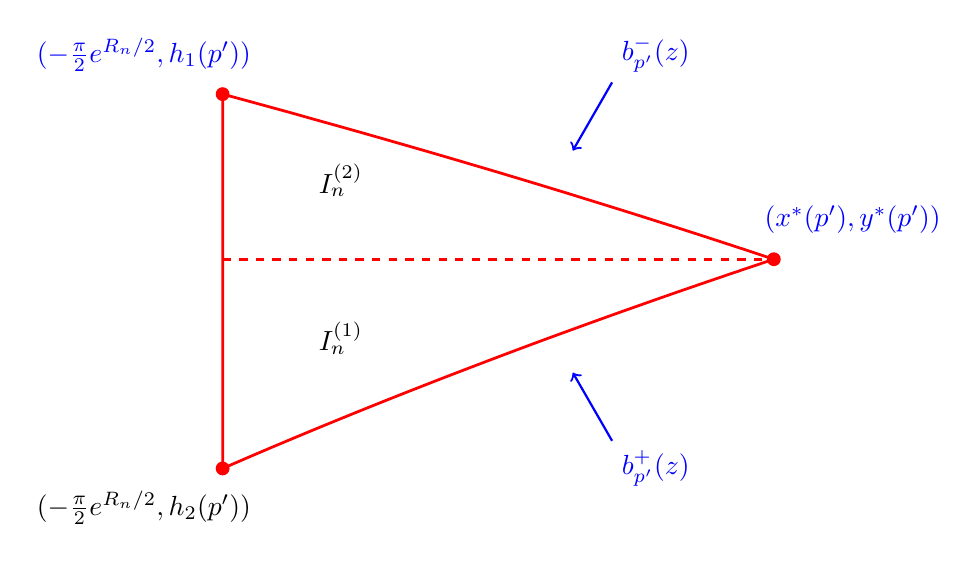
\begin{tikzpicture}[scale=5]

%%%%%%%%%%%%%%%%%%%%%%%%%%%%%%%%%%%%%%%%%%%%%%%%%%%%%%%%%%%%%%%%%%%%%%%%%%%%%%%%%%%%%%%%%%%%%%%%%%%
%																								  %
%	Shows the area T_{\Pcal \Delta \Pcal_n} when h_1(p^\prime) > h_2(p^\prime) > h(y)			  %
%																								  %
%%%%%%%%%%%%%%%%%%%%%%%%%%%%%%%%%%%%%%%%%%%%%%%%%%%%%%%%%%%%%%%%%%%%%%%%%%%%%%%%%%%%%%%%%%%%%%%%%%%

	%Define the coordinates 
	%p = (\u,\v) and p^\prime = (\uu, \vv)
	%Box \Rcal_n has width 2\r and height \t
	\pgfmathsetmacro{\u}{0}
	\pgfmathsetmacro{\v}{1}
	\pgfmathsetmacro{\uu}{1.4}
	\pgfmathsetmacro{\vv}{0.2}
	\pgfmathsetmacro{\r}{6}
	\pgfmathsetmacro{\t}{4}
    
    %Define x^\ast(p^\prime) and y^\ast(p^\prime)
    \pgfmathsetmacro{\uuast}{\uu-\r}
    \pgfmathsetmacro{\vvast}{2*ln(\r)-\vv}
    
    %Define intersection left black and shifted blue curve
    \pgfmathsetmacro{\vast}{2*ln((2*\r - \uu)/(exp(\v/2) + exp(\vv/2)))}
    \pgfmathsetmacro{\uast}{(\uu - 2*\r)/(1 + exp((\vv - \v)/2))}    
   
    %Define h_1(p) = h_2(p)
    \pgfmathsetmacro{\hp}{2*ln(\r-\u)-\v}
    
    %Define h_1(p^\prime) and h_2(p^\prime)
    \pgfmathsetmacro{\hh}{2*ln(\uu+\r)-\vv}
    \pgfmathsetmacro{\hhh}{2*ln(\r-\uu)-\vv}
    
    %Draw the boundary left black, left blue and shifted right blue line
	\draw[red,line width=1pt] 
		plot[domain=\uuast:-\r,smooth,variable=\x,red] (\x, {2*ln(\x+(2*\r-\uu))-\vv}) 
		-- 
		(-\r,\hh)
		-- 
		plot[domain=-\r:\uuast,smooth,variable=\x,red] (\x, {2*ln(\uu-\x)-\vv});
	
	\pgfmathsetmacro{\top}{2*ln(\uu-\uast)-\vv}
	
	\draw[red, dashed,line width=1pt] (-\r,\vvast) -- (\uuast,\vvast);

    \draw node at (-\r-0.2,\hh+0.1) {\color{blue}$(-\frac{\pi}{2} e^{R_n/2}, h_1(p^\prime))$};
    \draw node at (-\r-0.2,\hhh-0.1) {$(-\frac{\pi}{2} e^{R_n/2}, h_2(p^\prime))$};
    \draw node at (\uuast+0.2,\vvast+0.1) {\color{blue}$(x^\ast(p^\prime), y^\ast(p^\prime))$};
    
    \draw node at (-\r+0.3,\vvast+0.2) {$I_n^{(2)}$};
    \draw node at (-\r+0.3,\vvast-0.2) {$I_n^{(1)}$};
    
    \draw node (f2) at (\uuast-0.3,\hh+0.1) {\color{blue}$b_{p^\prime}^-(z)$};
    \draw node (f3) at (\uuast-0.3,\hhh) {\color{blue}$b_{p^\prime}^+(z)$};
    \path (f2)+(230:0.35) node (f2_arrow) {};
    \path (f3)+(130:0.35) node (f3_arrow) {};
    \draw[->,thick,blue] (f2.south west) -- (f2_arrow);
    \draw[->,thick,blue] (f3.north west) -- (f3_arrow);

	\draw node[red, fill, circle, inner sep=0pt, minimum size=5pt] at (-\r,\hhh) {};
	\draw node[red, fill, circle, inner sep=0pt, minimum size=5pt] at (-\r,\hh) {};
	\draw node[red, fill, circle, inner sep=0pt, minimum size=5pt] at (\uuast,\vvast) {};

\end{tikzpicture}\\
\vspace{20pt}
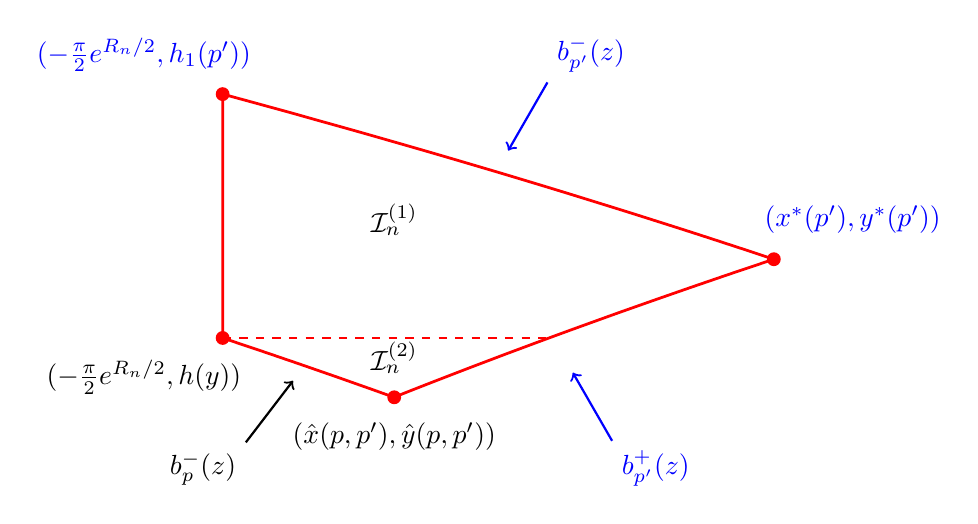
\begin{tikzpicture}[scale=5]
	%Define the coordinates 
	%p = (\u,\v) and p^\prime = (\uu, \vv)
	%Box \Rcal_n has width 2\r and height \t
	\pgfmathsetmacro{\u}{0}
	\pgfmathsetmacro{\v}{1}
	\pgfmathsetmacro{\uu}{1.4}
	\pgfmathsetmacro{\vv}{0.8}
	\pgfmathsetmacro{\r}{6}
	\pgfmathsetmacro{\t}{4}
    
    %Define x^\ast(p^\prime) and y^\ast(p^\prime)
    \pgfmathsetmacro{\uuast}{\uu-\r}
    \pgfmathsetmacro{\vvast}{2*ln(\r)-\vv}
    
    %Define intersection left black and shifted blue curve
    \pgfmathsetmacro{\vast}{2*ln((2*\r - \uu)/(exp(\v/2) + exp(\vv/2)))}
    \pgfmathsetmacro{\uast}{(\uu - 2*\r)/(1 + exp((\vv - \v)/2))}    
   
    %Define h_1(p) = h_2(p)
    \pgfmathsetmacro{\hp}{2*ln(\r-\u)-\v}
    
    %Define h_1(p^\prime) and h_2(p^\prime)
    \pgfmathsetmacro{\hh}{2*ln(\uu+\r)-\vv}
    \pgfmathsetmacro{\hhh}{2*ln(\r-\uu)-\vv}
    
    %Draw the boundary left black, left blue and shifted right blue line
	\draw[red,line width=1pt] 
		plot[domain=\uuast:\uast,smooth,variable=\x,red] (\x, {2*ln(\x+(2*\r-\uu))-\vv}) 
		-- 
		plot[domain=\uast:-\r,smooth,variable=\x,red] (\x, {2*ln(-\x)-\v})
		-- 
		(-\r,\hh)
		-- 
		plot[domain=-\r:\uuast,smooth,variable=\x,red] (\x, {2*ln(\uu-\x)-\vv});
	
	\pgfmathsetmacro{\rb}{\uu + exp((\vv+\hp)/2) -2*\r}
	

	%\draw[red,dashed,line width=1pt] (\uast,\vast) -- (\uast,\hp);
	\draw[red,dashed,line width=1pt] (-\r,\hp) -- (\rb,\hp);

    \draw node at (-\r-0.2,\hh+0.1) {\color{blue}$(-\frac{\pi}{2} e^{R_n/2}, h_1(p^\prime))$};
    \draw node at (-\r-0.2,\hp-0.1) {$(-\frac{\pi}{2} e^{R_n/2}, h(y))$};
    \draw node at (\uuast+0.2,\vvast+0.1) {\color{blue}$(x^\ast(p^\prime), y^\ast(p^\prime))$};
    \draw node at (\uast,\vast-0.1) {$(\hat{x}(p,p^\prime), \hat{y}(p, p^\prime))$};
    
    \draw node at (\uast,\vvast+0.1) {$\mathcal{I}_n^{(1)}$};
    \draw node at (\uast,\hp-0.05) {$\mathcal{I}_n^{(2)}$};
    %\draw node at (\uast+0.1,\hp-0.05) {$\mathcal{I}_n^{(3)}$};
    
    \draw node (f1) at (-\r-0.05,\hhh) {$b_p^-(z)$};
    \draw node (f2) at (\uast+0.5,\hh+0.1) {\color{blue}$b_{p^\prime}^-(z)$};
    \draw node (f3) at (\uuast-0.3,\hhh) {\color{blue}$b_{p^\prime}^+(z)$};
    \path (f1)+(45:0.35) node (f1_arrow) {};
    \path (f2)+(230:0.35) node (f2_arrow) {};
    \path (f3)+(130:0.35) node (f3_arrow) {};
    \draw[->,thick] (f1.north east) -- (f1_arrow);
    \draw[->,thick,blue] (f2.south west) -- (f2_arrow);
    \draw[->,thick,blue] (f3.north west) -- (f3_arrow);

	\draw node[red, fill, circle, inner sep=0pt, minimum size=5pt] at (-\r,\hp) {};
	\draw node[red, fill, circle, inner sep=0pt, minimum size=5pt] at (-\r,\hh) {};
	\draw node[red, fill, circle, inner sep=0pt, minimum size=5pt] at (\uuast,\vvast) {};
	\draw node[red, fill, circle, inner sep=0pt, minimum size=5pt] at (\uast,\vast) {};

\end{tikzpicture}\\
\vspace{20pt}
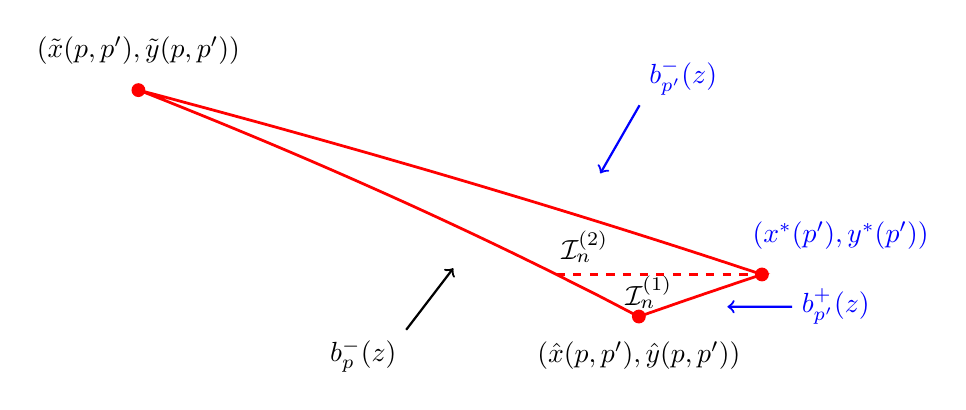
\begin{tikzpicture}[scale=5]

%%%%%%%%%%%%%%%%%%%%%%%%%%%%%%%%%%%%%%%%%%%%%%%%%%%%%%%%%%%%%%%%%%%%%%%%%%%%%%%%%%%%%%%%%%%%%%%%%%%
%																								  %
%	Shows the area T_{\Pcal \Delta \Pcal_n} when h(y) > h_1(p^\prime)							  %
%																								  %
%%%%%%%%%%%%%%%%%%%%%%%%%%%%%%%%%%%%%%%%%%%%%%%%%%%%%%%%%%%%%%%%%%%%%%%%%%%%%%%%%%%%%%%%%%%%%%%%%%%

	%Define the coordinates 
	%p = (\u,\v) and p^\prime = (\uu, \vv)
	%Box \Rcal_n has width 2\r and height \t
	\pgfmathsetmacro{\u}{0}
	\pgfmathsetmacro{\v}{1}
	\pgfmathsetmacro{\uu}{2.5}
	\pgfmathsetmacro{\vv}{1.8}
	\pgfmathsetmacro{\r}{6}
	\pgfmathsetmacro{\t}{4}
    
    %Define x^\ast(p^\prime) and y^\ast(p^\prime)
    \pgfmathsetmacro{\uuast}{\uu-\r}
    \pgfmathsetmacro{\vvast}{2*ln(\r)-\vv}
    
    %Define intersection left black and shifted blue curve
    \pgfmathsetmacro{\vast}{2*ln((2*\r - \uu)/(exp(\v/2) + exp(\vv/2)))}
    \pgfmathsetmacro{\uast}{(\uu - 2*\r)/(1 + exp((\vv - \v)/2))}    
    
    %Define intersection left black and left blue curve
    \pgfmathsetmacro{\utilde}{\uu/(1-exp((\vv-\v)/2))} 
    \pgfmathsetmacro{\vtilde}{2*ln(\uu-\utilde)-\vv}
   
    %Define h_1(p) = h_2(p)
    \pgfmathsetmacro{\hp}{2*ln(\r-\u)-\v}
    
    %Define h_1(p^\prime) and h_2(p^\prime)
    \pgfmathsetmacro{\hh}{2*ln(\uu+\r)-\vv}
    \pgfmathsetmacro{\hhh}{2*ln(\r-\uu)-\vv}
    
    %Draw the boundary left black, left blue and shifted right blue line
	\draw[red,line width=1pt] 
		plot[domain=\utilde:\uuast,smooth,variable=\x,red] (\x, {2*ln(\uu-\x)-\vv})
		--
		plot[domain=\uuast:\uast,smooth,variable=\x,red] (\x, {2*ln(\x+(2*\r-\uu))-\vv})
		--
		plot[domain=\uast:\utilde,smooth,variable=\x,red] (\x, {2*ln(-\x)-\v}); 
	
	%Calculate intersection point
	\pgfmathsetmacro{\i}{-exp((\v+\vvast)/2)}
	\draw[red, dashed,line width=1pt] (\i,\vvast) -- (\uuast,\vvast);

    \draw node at (\utilde,\vtilde+0.1) {\color{black}$(\tilde{x}(p,p^\prime), \tilde{y}(p,p^\prime))$};
    \draw node at (\uast,\vast-0.1) {$(\hat{x}(p,p^\prime), \hat{y}(p,p^\prime))$};
    \draw node at (\uuast+0.2,\vvast+0.1) {\color{blue}$(x^\ast(p^\prime), y^\ast(p^\prime))$};
   
    \draw node at (\uuast-0.45,\vvast+0.07) {$\mathcal{I}_n^{(2)}$};
    \draw node at (\uast+0.025,\vvast-0.045) {$\mathcal{I}_n^{(1)}$};
   
    \draw node (f1) at (\uast-0.7,\vast-0.1) {\color{black}$b_{p}^-(z)$};
    \draw node (f2) at (\uuast-0.2,\vvast+0.5) {\color{blue}$b_{p^\prime}^-(z)$};
    \draw node (f3) at (\uast+0.5,\vast+0.025) {\color{blue}$b_{p^\prime}^+(z)$};
    \path (f1)+(45:0.35) node (f1_arrow) {};
    \path (f2)+(230:0.35) node (f2_arrow) {};
    \path (f3)+(180:0.3) node (f3_arrow) {};
	\draw[->,thick] (f1.north east) -- (f1_arrow);
    \draw[->,thick,blue] (f2.south west) -- (f2_arrow);
    \draw[->,thick,blue] (f3.west) -- (f3_arrow);
%
	\draw node[red, fill, circle, inner sep=0pt, minimum size=5pt] at (\utilde,\vtilde) {};
	\draw node[red, fill, circle, inner sep=0pt, minimum size=5pt] at (\uast,\vast) {};
	\draw node[red, fill, circle, inner sep=0pt, minimum size=5pt] at (\uuast,\vvast) {};

\end{tikzpicture}
\caption{The different shapes of $\mathcal{T}_{\Pcal \Delta \Pcal_n}(p,p_1)$ depending on the regime to which $p_1$ belongs. The top figure is for $p_1 \in B_n^{(1)}$, the middle for $p_1 \in B_n^{(2)}$ and the bottom one for $p_1 \in B_n^{(3)}$.}
\label{fig:shapes_triangle_mismatches}
\end{figure}

\paragraph{Regime 1: $0 \le y_1 \le y - 2\log(I_n/(I_n-x_1))$}

In this case the integral over $p_2$ splits into two parts
\begin{align*}
	\mathcal{I}_n^{(1)}(p_1) &:= \int_{h_2(p_1)}^{y^\ast(p_1)} \int_{-I_n}^{x_1 + e^{(y_1+y_2)/2}-2I_n} e^{-\alpha y_2}
		\dd x_2 \dd y_2\\
	\mathcal{I}_n^{(2)}(p_1) &:= \int_{y^\ast(p_1)}^{h_1(p_1)} \int_{x^\ast(p_1)}^{x_1 - e^{(y_1+y_2)/2}} e^{-\alpha y_2}
		\dd x_2 \dd y_2.
\end{align*}

We first compute $\mathcal{I}_n^{(1)}$.
\begin{align*}
	\mathcal{I}_n^{(1)}(p_1) &= \int_{h_2(p_1)}^{y^\ast(p_1)} \left(x_1 + e^{(y_1+y_2)/2} - I_n\right) e^{-\alpha y_2} 
		\dd x_2 \dd y_2\\
	&\le e^{y_1/2} \int_{h_2(p_1)}^{y^\ast(p_1)} e^{-(\alpha-\frac{1}{2}) y_2} \dd y_2\\
	&= \frac{2 e^{y_1/2}}{2\alpha - 1} \left(e^{-(\alpha-\frac{1}{2})h_2(p_1)} - e^{-(\alpha-\frac{1}{2})y^\ast(p_1)}
		\right) \\
	&= \frac{2 e^{\alpha y_1}}{2\alpha - 1} I_n^{-(2\alpha -1)}\left(\left(1 - \frac{x_1}{I_n}\right)^{-(2\alpha - 1)}-1\right)\\
	&= \bigO{I_n^{-2\alpha} x_1 e^{\alpha y_1}},
\end{align*}
where we used that $x^\prime \le e^{(y+y_1)/2} = \smallO{I_n}$ for all $y_1\le y$ and $y \in \Kcal_{C}(k_n)$ so that
\[
	\left(\left(1 - \frac{x_1}{I_n}\right)^{-(2\alpha - 1)}-1\right) = \bigO{\frac{x^\prime}{I_n}} \quad 
	\text{as } n \to \infty.
\]

For $\mathcal{I}_n^{(2)}(p_1)$ we have
\begin{align*}
	\mathcal{I}_n^{(2)}(p_1) &= \int_{y^\ast(p_1)}^{h_1(p_1)} \left(I_n + x_1 - e^{(y_1+y_2)}\right) e^{-\alpha y_2}
		\dd x_2 \dd y_2\\
	&\le 2 I_n \int_{y^\ast(p_1)}^{h_1(p_1)} e^{-\alpha y_2} \dd x_2 \dd y_2\\
	&= \frac{2}{\alpha} I_n \left(I_n^{-2\alpha}e^{\alpha y_1} - \left(I_n + x_1\right)^{-2\alpha} e^{-\alpha y_1}\right)\\
	&= \bigO{I_n^{-2\alpha} x_1 e^{\alpha y_1}} = \bigO{I_n^{-(2\alpha - 1)} e^{\alpha y_1}}.
\end{align*}

We conclude that for $p_1 \in B_n^{(1)}$:
\[
	\mu_{\alpha, \nu}\left(\mathcal{T}_{\Pcal \Delta \Pcal_n}(p,p_1)\right) = \bigO{I_n^{-2\alpha} x_1 e^{\alpha y_1}},
\]
which establishes the first part of \eqref{eq:mu_triangle_diff}.

\paragraph{Regime 2: $y - 2\log(I_n/(I_n-x_1)) < y_1 \le y + 2 \log\left(1 + \frac{x_1}{I_n}\right)$}

Here we split the integration into two parts (see Figure~\ref{fig:shapes_triangle_mismatches}). Recall that $x^\ast(p,p_1) = x_1 - I_n$. Then, for the first part we have
\begin{align*}
	\mathcal{I}_n^{(1)}(p,p_1) &\le \int_{h(y)}^{h_1(p_1)} \int_{-I_n}^{x^\ast(p,p_1)} f_{\alpha,\nu}(x_2, y_2) 
		\dd x_2 \dd y_2\\
	&= \bigO{x_1 \left(e^{-\alpha h(y)} - e^{-\alpha h_1(p_1)}\right)}\\
	&= \bigO{x_1 I_n^{-2\alpha}\left(e^{\alpha y} - e^{\alpha y_1}\left(1 + \frac{x_1}{I_n}\right)^{-2\alpha}\right)}\\
	&= \bigO{I_n^{-2\alpha} x_1 e^{\alpha y_1}\left(\left(1 - \frac{x_1}{I_n}\right)^{-2\alpha} 
		- \left(1 + \frac{x_1}{I_n}\right)^{-2\alpha}\right)}\\
	&= \bigO{I_n^{-2\alpha} x_1 e^{\alpha y_1}} = \bigO{I_n^{-(2\alpha - 1)} e^{\alpha y}}, 
\end{align*}
were we used that $y \le y_1 + 2\log(I_n/(I_n-x_1))$ for $p_1 \in B_n^{(2)}$ for the third line and 
\[
	\left(1 - \frac{x_1}{I_n}\right)^{-2\alpha} - \left(1 + \frac{x_1}{I_n}\right)^{-2\alpha}
	= \bigO{\frac{x_1}{I_n}} = \bigO{1},
\]
for the last line.

For the second part we first compute that 
\begin{align*}
	x_1 + e^{(y_1+y_2)/2} - 2 I_n + e^{(y + y_2)/2} &\le \left(e^{y/2} + e^{y_1/2}\right)e^{y_2/2}\\
	&\le e^{y/2}\left(1 + \frac{I_n}{I_n - e^y}\right)e^{y_2/2} = \bigO{e^{(y+y_2)/2}},
\end{align*}
since $y \in \Kcal_{C}(k_n)$ and $k_n = \smallO{\sqrt{n}}$, so that $e^y = \smallO{n} = \smallO{I_n}$. 
Then we have
\begin{align*}
	\mathcal{I}_n^{(2)} &= \int_{\hat{y}(p,p_1)}^{h(y)} \int_{-e^{(y + y_2)/2}}^{x_1 + e^{(y+y_1)/2} - 2 I_n} 
		f_{\alpha,\nu}(x_2, y_2) \dd x_2 \dd y_2\\
	&= \bigO{e^{y/2} \int_{\hat{y}(p,p_1)}^{h(y)} e^{-(\alpha -\frac{1}{2}) y_2} \dd y_2}\\
	&= \bigO{e^{y/2} \left(e^{-(\alpha -\frac{1}{2}) \hat{y}(p,p_1)} - e^{-(\alpha -\frac{1}{2}) h(y)}\right)}\\
	&= \bigO{e^{y/2} \left(\left(\frac{2I_n - x_1}{e^{y/2} + e^{y_1/2}}\right)^{-(2\alpha-1)} 
		- I_n^{-(2\alpha-1)} e^{(\alpha -\frac{1}{2}) y}\right)}\\
	&= \bigO{I_n^{-(2\alpha-1)} e^{\alpha y}},
\end{align*}
where for the last line we first used that $(2I_n - x_1)^{-(2\alpha-1)} \le I_n^{-(2\alpha-1)}$ and then
\[
	\left(\left(e^{y/2} + e^{y_1/2}\right)^{2\alpha-1}- e^{(\alpha -\frac{1}{2}) y}\right)
	\le e^{(\alpha -\frac{1}{2}) y}\left(\left(1 + \sqrt{1+\frac{x_1}{I_n}} \, \right)^{2\alpha - 1} - 1\right)
	= \bigO{e^{(\alpha -\frac{1}{2}) y}}.
\]

It then follows that for $p_1 \in B_n^{(2)}$
\[
	\mu_{\alpha, \nu}\left(\mathcal{T}_{\Pcal \Delta \Pcal_n}(p,p_1)\right) = \bigO{I_n^{-(2\alpha-1)} e^{\alpha y}}.
\]

\paragraph{Regime III $\bm{p_1 \in B_n^{(3)}}$:}

\begin{align*}
	\mathcal{I}_n^{(1)} &= \int_{y^\ast}^{\tilde{y}} \int_{-e^{(y+y_2)/2}}^{x_1-e^{(y_1+y_2)/2}} f_{\alpha, \nu}(x_2,y_2)
		\dd x_2 \dd y_2\\
	&= \bigO{\int_{y^\ast}^{\tilde{y}} x_1 e^{-\alpha y_2} - \left(e^{y_1/2} - e^{y/2}\right)e^{-(\alpha - \frac{1}{2})y_2}
		\dd y_2}\\
	&= \bigO{x_1 \int_{y^\ast}^{\tilde{y}}  e^{-\alpha y_2} \dd y_2}.
\end{align*}

Now 
\begin{align*}
	\int_{y^\ast}^{\tilde{y}}  e^{-\alpha y_2} \dd y_2 
	&= \frac{1}{\alpha}\left(e^{-\alpha y^\ast} - e^{-\alpha \tilde{y}}\right) 
		= \frac{1}{\alpha}\left(I_n^{-2\alpha} e^{\alpha y_1} 
		- \left(\frac{x_1}{e^{y_1/2} - e^{y/2}}\right)^{-2\alpha}\right) \\
	&= \frac{I_n^{-2\alpha} e^{\alpha y_1}}{\alpha}\left(1 - \left(1 - e^{(y - y_1)/2}\right)^{2\alpha}
		\left(\frac{x_1}{I_n}\right)^{-2\alpha}\right) = \bigO{I_n^{-2\alpha} e^{\alpha y_1}},
\end{align*}
and hence we have
\[
	\mathcal{I}_n^{(1)} = \bigO{I_n^{-2\alpha} x_1 e^{\alpha y_1}}.
\]

For the second integral we have
\begin{align*}
	\mathcal{I}_n^{(2)} &= \int_{\hat{y}}^{y^\ast} \int_{-e^{(y+y_2)/2}}^{e^{(y_1 + y_2)/2} + x_1 - 2I_n} 
		f_{\alpha, \nu}(x_2,y_2)\dd x_2 \dd y_2\\
	&= \bigO{\int_{\hat{y}}^{y^\ast} \left(e^{y/2} + e^{y_1/2}\right)e^{-(\alpha - \frac{1}{2})y_2} \dd y_2}\\
	&= \bigO{ e^{y_1/2} \int_{\hat{y}}^{y^\ast}e^{-(\alpha - \frac{1}{2})y_2} \dd y_2}.
\end{align*}

For the integral we have
\begin{align*}
	\int_{\hat{y}}^{y^\ast}e^{-(\alpha - \frac{1}{2})y_2} \dd y_2
	&= \frac{2}{2\alpha - 1} \left(e^{-(\alpha - \frac{1}{2})\hat{y}} - e^{-(\alpha - \frac{1}{2})y^\ast}\right)\\
	&= \frac{2}{2\alpha - 1}\left(\left(\frac{2I_n - x_1}{e^{y/2} + e^{y_1/2}}\right)^{-(2\alpha - 1)} 
		- I_n^{-(2\alpha - 1)} e^{-(\alpha - \frac{1}{2})y_1}\right)\\
	&= \bigO{I_n^{-2\alpha} x_1 e^{-(\alpha - \frac{1}{2})y_1}}
\end{align*}
so that
\[
	\mathcal{I}_n^{(2)} = \bigO{I_n^{-(2\alpha - 1)} e^{(1-\alpha)y_1}} = \bigO{I_n^{-2\alpha} x_1 e^{\alpha y}}
\]
and hence for $p_1 \in B_n^{(3)}$
\[
	\mu_{\alpha, \nu}\left(\mathcal{T}_{\Pcal \Delta \Pcal_n}(p,p_1)\right) = \bigO{I_n^{-2\alpha} x_1 e^{\alpha y}}
	= \bigO{I_n^{-(2\alpha - 1)} e^{\alpha y}}.
\]

\subsubsection*{Integration over $p_1$}



We now proceed with the second part of the computation leading to \eqref{eq:clustering_error_T_main}. Here we will integrate $\mu_{\alpha, \nu}(\mathcal{T}_{\Pcal \Delta \Pcal_n})(p,p_1)$ over the region $B_n := B_n^{(1)} \cup B_n^{(2)} \cup B_n^{(3)}$, see Figure~\ref{fig:comparing_triangles_B_areas}. Let us first identify the boundaries of these areas. 

The area $B_n^{(1)}$ is bounded from above by the line given by the equation
\[
	y_1 = y - 2\log\left(\frac{I_n}{I_n - x_1}\right).
\]
Solving this for $x_1$ yields $x_1 = I_n\left(1 - e^{(y_1-y)/2}\right)$ and hence the area $B_n^{(1)}$ is given by
\[
	B_n^{(1)} = \left\{(x_1, y_1) \, : \, 0 \le y_1 \le y, \quad 0 \le x_1 \le I_n\left(1 - e^{(y_1-y)/2}\right) \wedge e^{(y + y_1)/2} \right\}.
\]

In a similar way we have that $B_n^{(2)}$ is bounded from above by line
\[
	y_1 = y + 2\log\left(\frac{I_n}{I_n + x_1}\right),
\]
which yields $x_1 = I_n\left(e^{(y_1 - y)/2} - 1\right)$. The lower red boundary is the upper boundary of $B_n^{(2)}$ and hence we have
\[
	B_n^{(2)} = \left\{(x_1, y_1) \, : \, h_\ast(y) \le y_1 \le h^\ast(y), \,\, I_n\left(1 - e^{(y_1-y)/2}\right) \vee 
	I_n\left(e^{(y_1 - y)/2} - 1\right) \le x_1 \le e^{(y + y_1)/2} \right\}.
\]

We continue is the same way to obtain for $B_n^{(3)}$
\[
	B_n^{(3)} = \left\{(x_1, y_1) \, : \, y \le y_1 \le R_n, \,\,
	I_n\left(1 - e^{(y - y_1)/2}\right) \le x_1 \le I_n\left(e^{(y_1 - y)/2} - 1\right) \wedge e^{(y + y_1)/2} \wedge I_n \right\}.
\]

We these characterizations of the areas we now integrate $\mu_{\alpha, \nu}(\mathcal{T}_{\Pcal \Delta \Pcal_n})(p,p_1)$ over $B_n$, splitting the computations over the three different areas.

\paragraph{$\bm{p_1 \in B_n^{(1)}}:$}

We use that $I_n\left(1 - e^{(y_1-y)/2}\right) \wedge e^{(y + y_1)/2} \le I_n\left(1 - e^{(y_1-y)/2}\right)$ so that
\begin{align*}
	&\hspace{-30pt}\int_{B_n^{(1)}} \mu_{\alpha, \nu}\left(\mathcal{T}_{\Pcal \Delta \Pcal_n}(p,p_1)\right) 
		f_{\alpha,\nu}(x_1,y_1)	\dd x_1 \dd y_1 \\
	&\le  \int_0^y \int_0^{I_n(1-e^{(y_1-y)/2})} \mu_{\alpha, \nu}\left(\mathcal{T}_{\Pcal \Delta \Pcal_n}(p,p_1)\right) 
		f_{\alpha,\nu}(x_1,y_1) \dd x_1 \dd y_1\\
	&= \bigO{ I_n^{-2\alpha} \int_0^y \int_0^{e^{(y+y_1)/2}}  x_1 \dd x_1 \dd y_1 }\\
	&= \bigO{I_n^{-(2\alpha-1)} \int_0^y \left(1 - e^{(y_1-y)/2}\right)^2 \dd y_1} \\
	&= \bigO{I_n^{-(2\alpha - 1)} y} = \bigO{y n^{-(2\alpha - 1)}}.
\end{align*} 

\paragraph{$\bm{p_1 \in B_n^{(2)}}:$}

We will show that
\begin{equation}\label{eq:mu_triangle_diff_2}
	\mu_{\alpha, \nu}(B_n^{(2)}) = \bigO{I_n^{-1} e^{(2-\alpha)y}},
\end{equation}
which together with \eqref{eq:mu_triangle_diff} yields
\begin{align*}
	\int_{B_n^{(2)}} \mu_{\alpha, \nu}\left(\mathcal{T}_{\Pcal \Delta \Pcal_n}(p,p_1)\right) 
		f_{\alpha,\nu}(x_1,y_1)	\dd x_1 \dd y_1
	&= \bigO{\mu_{\alpha, \nu}(B_n^{(2)}) I_n^{-(2\alpha - 1)} e^{\alpha y}}\\
	&= \bigO{I_n^{-2\alpha} e^{2y}}.
\end{align*}

The integration is split into two parts determined by $I_n\left(1 - e^{(y_1-y)/2}\right) \vee 
	I_n\left(e^{(y_1 - y)/2} - 1\right)$:
\begin{align*}
	\mu_{\alpha, \nu}(B_n^{(3)}) &= \int_{h_\ast(y)}^{y} \int_{I_n(1-e^{(y_1-y)/2})}^{e^{(y + y_1)/2}} 
		f_{\alpha,\nu}(x_1,y_1) \dd x_1 \dd y_1\\
	&\hspace{10pt} + \int_y^{h^\ast(y)} \int_{I_n(e^{(y_1-y)/2}-1)}^{e^{(y + y_1)/2}} 
		f_{\alpha,\nu}(x_1,y_1) \dd x_1 \dd y_1.
\end{align*}

For the first integral we use that $e^{(y + y_1)/2} - I_n(1-e^{(y_1-y)/2}) \le e^{y_1/2}\left(e^{y/2} + e^{-y/2}\right)$ to obtain
\begin{align*}
	&\hspace{-30pt}\int_{h_\ast(y)}^{y} \int_{I_n(1-e^{(y_1-y)/2})}^{e^{(y + y_1)/2}} f_{\alpha,\nu}(x_1,y_1) 
		\dd x_1 \dd y_1\\
	&= \bigO{e^{y/2} \int_{h_\ast(y)}^{y} e^{-(\alpha - \frac{1}{2})y_1} \dd y_1}\\
	&= \bigO{e^{y/2}\left(e^{-(\alpha - \frac{1}{2})y} - e^{-(\alpha - \frac{1}{2})y} 
		\left(\frac{I_n}{I_n + e^y}\right)^{-(2\alpha - 1)}\right)}\\
	&= \bigO{I_n^{-1} e^{(2-\alpha)y}}.
\end{align*}
For the second integral note that $e^{(y + y_1)/2} - I_n(e^{(y_1-y)/2}-1) \le e^{(y + y_1)/2}$ and hence
\begin{align*}
	&\hspace{-30pt}\int_y^{h^\ast(y)} \int_{I_n(e^{(y_1-y)/2}-1)}^{e^{(y + y_1)/2}} f_{\alpha,\nu}(x_1,y_1) 
		\dd x_1 \dd y_1\\
	&= \bigO{e^{y/2} \int_y^{h^\ast(y)} e^{-(\alpha - \frac{1}{2})y_1} \dd y_1}\\
	&= \bigO{e^{y/2} \left(e^{-(\alpha - \frac{1}{2})y} - e^{-(\alpha - \frac{1}{2})y}
		\left(\frac{I_n}{I_n - e^y}\right)^{-(2\alpha - 1)}\right)}\\
	&= \bigO{I_n^{-1} e^{(2-\alpha)y}},
\end{align*}
so that \eqref{eq:mu_triangle_diff_2} follows.

\paragraph{$\bm{p_1 \in B_n^{(3)}}:$}

For this area we show that 
\begin{equation}\label{eq:mu_triangle_diff_3}
	\mu_{\alpha, \nu}(B_n^{(3)}) = \bigO{e^{(1-\alpha)y}}
\end{equation} 
so that
\begin{align*}
	\int_{B_n^{(3)}} \mu_{\alpha, \nu}\left(\mathcal{T}_{\Pcal \Delta \Pcal_n}(p,p_1)\right) 
		f_{\alpha,\nu}(x_1,y_1)	\dd x_1 \dd y_1
	&= \bigO{\mu_{\alpha, \nu}(B_n^{(2)}) I_n^{-(2\alpha - 1)} e^{\alpha y}}\\
	&= \bigO{I_n^{-(2\alpha-1)} e^{y}}.
\end{align*}

Here the integral is split into three parts:
\begin{align*}
	\mu_{\alpha, \nu}(B_n^{(3)}) &= \int_y^{h^\ast(y)} \int_{I_n(1-e^{(y-y_1)/2})}^{I_n(e^{(y_1-y)/2}-1)}
		f_{\alpha,\nu}(x_1,y_1) \dd x_1 \dd y_1\\
	&\hspace{10pt}+ \int_{h^\ast(y)}^{h(y)} \int_{I_n(1-e^{(y-y_1)/2})}^{e^{(y+y_1)/2}}
		f_{\alpha,\nu}(x_1,y_1) \dd x_1 \dd y_1\\
	&\hspace{10pt}+ \int_{h(y)}^{R_n} \int_{I_n(1-e^{(y-y_1)/2})}^{I_n}
		f_{\alpha,\nu}(x_1,y_1) \dd x_1 \dd y_1.
\end{align*}

Let us first focus on the first integral. Since	$I_n(e^{(y_1-y)/2}-1) - I_n(1-e^{(y-y_1)/2}) \le I_n e^{(y_1-y)/2}$ we get,
using similar arguments as above
\begin{align*}
	\int_y^{h^\ast(y)} \int_{I_n(1-e^{(y-y_1)/2})}^{I_n(e^{(y_1-y)/2}-1)} f_{\alpha,\nu}(x_1,y_1) \dd x_1 \dd y_1
	&= \bigO{I_n e^{-y/2} \int_y^{h^\ast(y)} e^{-(\alpha - \frac{1}{2})y_1} \dd y_1}\\
	&= \bigO{I_n e^{-\alpha y} \left(1 - \left(\frac{I_n}{I_n - e^y}\right)^{-(2\alpha - 1)}\right)}\\
	&= \bigO{e^{(1-\alpha)y}}.
\end{align*}

Proceeding to the second integral, we first note that $e^{(y+y_1)/2} - I_n(1-e^{(y-y_1)/2}) = \bigO{I_n e^{(y_1-y)/2}}$ so that similar calculations as before yield
\begin{align*}
	\int_{h^\ast(y)}^{h(y)} \int_{I_n(1-e^{(y-y_1)/2})}^{e^{(y+y_1)/2}}	f_{\alpha,\nu}(x_1,y_1) \dd x_1 \dd y_1
	&= \bigO{I_n e^{-y/2} \int_{h^\ast(y)}^{h(y)} e^{-(\alpha - \frac{1}{2})y_1} \dd y_1}
		= \bigO{e^{(1-\alpha)y}}.
\end{align*}



\end{proof}